\section{Polynomial maximum depth with rank-subset scheduling}
\label{sec:polynomial-slots}

The direct maximum-depth guarantee in
Section~\ref{sec:quasipolynomial} can be obtained in polynomial time.
The key is an exact interval-deadline algorithm exponential in the
\emph{total number of schedule slots}, rather than in the number of
distinct deadline grades. Restrict this algorithm to a logarithmic
number of slots and retain the priority schedule as a fallback.
Two simultaneous recursive bounds then cover all instances.
The algorithm checks schedules against the heights of its own stored
children. An optimal witness path is used only to prove that a passing
schedule exists; neither that path nor its optimum height is an input.

\subsection{Exact interval deadlines with a bounded number of ranks}

Algorithm~\ref{alg:slot-dp} specifies the rank-subset DP, and
Algorithm~\ref{alg:hybrid-tree} gives the capped recursion.
Candidates are the integers $1,\ldots,M$. A demand is an interval
$[a,b]$ with an integer deadline $d_{[a,b]}$: some selected candidate
in that interval must occur by rank $d_{[a,b]}$. Selected candidates
are distinct, and the total schedule length is at most $L$.

\begin{lemma}[Rank-subset interval scheduling]
\label{lem:rank-subset-scheduling}
Interval-deadline feasibility and a feasible schedule can be computed
in $O(M^3 3^L+NM^2)$ time with $O(M^2 2^L)$ dynamic-programming
states, where $N$ is the number of demands. For circular intervals,
enumerating the first candidate adds a factor $M$.
\end{lemma}
\begin{proof}
For a spatial region $[l,r]$, let $\mathcal I(l,r)$ contain precisely
the original demands wholly inside that region. These are exactly
the demands still unhit: a demand crossing an earlier separator was
hit there, whereas a contained demand contains no earlier separator.
A state
$F(l,r,T)$, with $T\subseteq\{1,\ldots,L\}$, asks whether those
demands can be hit using candidates in $[l,r]$ assigned distinct
absolute ranks from $T$. Ranks may remain unused.
Keeping their absolute values allows queries in the left and right
regions to be interleaved without losing either region's deadlines.

If $\mathcal I(l,r)$ is empty, the state is true. If it is nonempty
and $T$ is empty, the state is false. Otherwise put $t=\min T$;
reject if any contained demand has deadline less than $t$. Enumerate
a candidate $p\in[l,r]$ and a partition
$T\setminus\{t\}=T_L\mathbin{\dot\cup}T_R$. Accept if
\[
 F(l,p-1,T_L)\quad\hbox{and}\quad F(p+1,r,T_R)
\]
both accept. Candidate $p$ is queried at rank $t$. All demands
containing it are now hit; every remaining demand is wholly inside
exactly one child region.

The earliest available rank can always be used: move the first query
of any feasible state to $\min T$, which only accelerates hits.
The resulting recursion is the spatial Cartesian tree of a schedule,
whose root is its earliest query. Its left and right descendants
partition the remaining assigned ranks, giving a successful transition.
Conversely, a successful recurrence
assigns distinct ranks meeting every deadline. Reconstruction sorts
the selected points by rank and deletes unused slots, again only
accelerating hits.

The existence and minimum deadline of contained demands can be
precomputed in $O(NM^2)$ time. There are $O(M^2 2^L)$ states, and
the total number of rank partitions over all masks is bounded by
$\sum_T2^{|T|}=3^L$. Trying $M$ root candidates gives the stated time.
For a circular instance, enumerate its first selected candidate,
discard the demands it hits, and cut the circle there. All surviving
demands are ordinary intervals. Subtract one from their deadlines and
use $L-1$ slots. A surviving demand with deadline at most one rejects
that trial. Enumerating the first candidate is exact.
\end{proof}

\begin{algorithm}[H]
\caption{\SlotDP: exact interval deadlines with a rank subset}
\label{alg:slot-dp}
\KwIn{Ordinary interval demands and deadlines; region $[l,r]$;
available absolute ranks $T\subseteq[L]$.}
\KwOut{A feasible rank assignment, or infeasible.}
\If{no original demand is wholly contained in $[l,r]$}{\KwRet the empty assignment\;}
\If{$T=\varnothing$}{\KwRet infeasible\;}
\If{this state is memoized}{\KwRet its stored result\;}
$t\gets\min T$\;
\If{a wholly contained demand has deadline $<t$}{\KwRet infeasible\;}
\ForEach{$p\in[l,r]$ and $T_L\subseteq T\setminus\{t\}$}{
  $T_R\gets T\setminus(T_L\cup\{t\})$\;
  Recurse on $([l,p-1],T_L)$ and $([p+1,r],T_R)$\;
  \If{both assignments are feasible}{
    Memoize their union with $(p,t)$ and \KwRet it\;
  }
}
Memoize and return infeasible\;
\end{algorithm}

Sort selected candidates by their ranks and suppress unused ranks.
The circular wrapper forces the first candidate, cuts there, and
subtracts one from surviving deadlines and the slot cap.
For the optional complete-exit variant, precompute the two oriented
decoder costs by Algorithm~\ref{alg:endpoint-code}; replace the deadline
precheck by the two local height tests of
Section~\ref{sec:polynomial-slots}. The same rank partitions apply.


\subsection{The hybrid recursive algorithm}

Use the rational count parameters of Section~\ref{sec:worst},
\[
 \delta=\frac{245122334}{10^9},\qquad
 \gamma=\frac{246496526}{10^8}.
\]
Let $n$ be the size of the \emph{original} instance and fix
\begin{equation}\label{eq:global-slot-cap}
 q=\lceil\log_2n\rceil,\qquad
 R=\left\lfloor\frac{\gamma q}{\gamma-1}\right\rfloor,
 \qquad L=R+1.
\end{equation}
This cap is retained throughout the recursion; it is not recomputed
from a child's size. Singleton states stop, and count-balanced states
use the existing balanced-query rule.

At a count-flat state $S$, build each full hull-pattern child's
\emph{hybrid} code once and record its actual height $C_W(A)$.
For each trial height $H$, consider both the existing priority
construction and a capped exact adjacent-block construction. Choose
the least passing trial over the two alternatives. Both use the same
already-built child codes.
The priority alternative guarantees that some trial passes. The exact
alternative can improve that trial when a short comparison schedule
exists; the algorithm tries it without testing the unknown optimum.

For the exact alternative, candidate blocks are edges of the full
normalized hull, retaining the origin as a free negative marker when
it is a hull vertex. Every nonzero pattern induces a circular interval
of blocks that meet its positive vertex arc. Put $s=|S|$ and
\[
 z_A=\lfloor\log_2(\delta s/|A|)\rfloor,\qquad
 B_A=\left\lfloor\frac{H-C_W(A)-z_A-5}{2}\right\rfloor.
\]
Reject negative budgets, assign deadline $B_A+1$ to class $A$, and
cap the total number of blocks at
\begin{equation}\label{eq:hybrid-total-cap}
 \min\{L,\lfloor H/2\rfloor\}.
\end{equation}
Apply Lemma~\ref{lem:rank-subset-scheduling}, including enumeration
of the first block. There is no deadline rounding. Execute the
resulting blocks, omitting cached endpoint tests, and attach the
existing endpoint codes and child codes. The adjacent-block allowance
\eqref{eq:qp-block-allowance} is
\begin{equation}\label{eq:slot-block-allowance}
 2(k-1)+z_A+5+C_W(A)
\end{equation}
when $A$ first meets block $k$. Thus every passing positive exit fits
$H$, by the same route decomposition as
Lemma~\ref{lem:worst-local-height}. The total cap pays for at most
$2\lfloor H/2\rfloor\le H$
queries on the all-negative route, identifying the zero singleton
when present. An infeasible all-negative leaf is omitted otherwise.
The low-dimensional hull case uses its at most two real extreme tests
directly, as in the preceding constructions.

Trial heights need only reach $\lfloor(3+\gamma)(s-1)\rfloor$,
since the priority alternative will have a passing trial. Computing
$q$ and $z_A$ uses integer powers of two and rational comparisons;
$R$ is the floor of a fixed rational multiple of $q$.
All algorithmic decisions have polynomial bit complexity.

\begin{algorithm}[H]
\caption{\HybridTree: general polynomial maximum depth}
\label{alg:hybrid-tree}
\KwIn{State $S$, original size $n$, fixed global cap
$L=R+1$, where $q=\lceil\log_2 n\rceil$ and $R=\lfloor\gamma q/(\gamma-1)\rfloor$,
and the count parameters of Section~\ref{sec:worst}.}
\KwOut{A tree satisfying Theorem~\ref{thm:poly-slot-worst}.}
Stop at a singleton; at a count-balanced state query a balanced line and recurse\;
Compute $\HullData(S)$ and build each child's hybrid code once\;
Handle a low-dimensional hull directly; otherwise record child heights $h_A$\;
\For{$H=1,\ldots,\lfloor(3+\gamma)(|S|-1)\rfloor$}{
  Try $\PriorityTrial$ with these stored children\;
  Set $z_A=\lfloor\log_2(\delta|S|/|A|)\rfloor$ and
  $B_A=\lfloor(H-h_A-z_A-5)/2\rfloor$\;
  \If{all $B_A\ge0$}{
    Try circular $\SlotDP$ on full-hull-edge demands with deadlines $B_A+1$
    and slot cap $\min\{L,\lfloor H/2\rfloor\}$\;
    Optionally also try the complete-exit version of $\SlotDP$\;
  }
  \If{any alternative passes}{
    Attach its endpoint decoders and the stored child trees\;
    Terminate the negative cover at $A_0$ when present; omit that leaf otherwise\;
    \KwRet a passing tree, contracting constant queries\;
  }
}
\end{algorithm}

The global cap is inherited unchanged by every child. The priority
fallback proves that a trial always passes; the algorithm never tests
the unknown condition $\OPT_W(S)\le R$.


\begin{figure}[htbp]
\centering
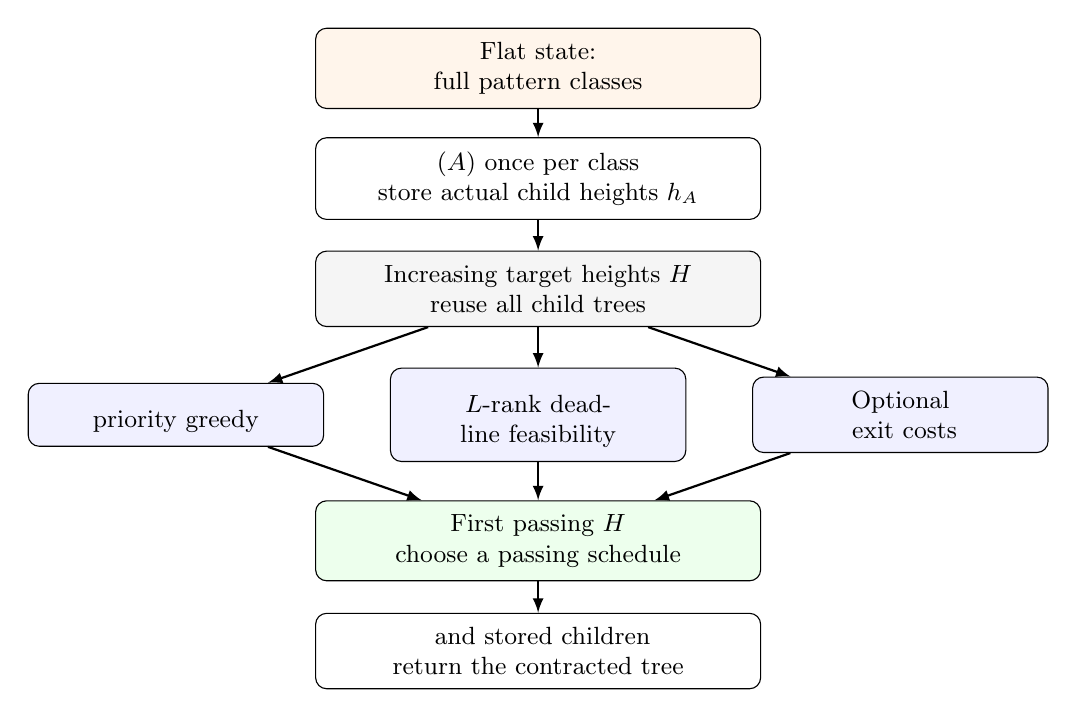
\begin{tikzpicture}[every node/.style={font=\small},
  box/.style={draw,rounded corners,align=center,inner sep=5pt,text width=3.4cm},
  wide/.style={box,text width=5.3cm},arr/.style={-latex,thick}]
  \node[wide,fill=orange!8] (hull) at (0,0)
    {Flat state: \HullData\\full pattern classes};
  \node[wide] (children) at (0,-1.4)
    {\HybridTree$(A)$ once per class\\store actual child heights $h_A$};
  \node[wide,fill=gray!8] (trial) at (0,-2.8)
    {Increasing target heights $H$\\reuse all child trees};
  \node[box,fill=blue!6] (priority) at (-4.6,-4.4)
    {\PriorityTrial\\priority greedy};
  \node[box,fill=blue!6] (slots) at (0,-4.4)
    {\SlotDP\\$L$-rank deadline feasibility};
  \node[box,fill=blue!6] (whole) at (4.6,-4.4)
    {Optional \SlotDP\\\EndpointCode\ exit costs};
  \node[wide,fill=green!7] (pass) at (0,-6)
    {First passing $H$\\choose a passing schedule};
  \node[wide] (attach) at (0,-7.4)
    {\EndpointCode\ and stored children\\return the contracted tree};
  \draw[arr] (hull) -- (children);
  \draw[arr] (children) -- (trial);
  \draw[arr] (trial) -- (priority);
  \draw[arr] (trial) -- (slots);
  \draw[arr] (trial) -- (whole);
  \draw[arr] (priority) -- (pass);
  \draw[arr] (slots) -- (pass);
  \draw[arr] (whole) -- (pass);
  \draw[arr] (pass) -- (attach);
\end{tikzpicture}
\caption{Construction of the polynomial maximum-depth tree at a flat
state. Arrows pass explicitly computed geometry, heights, or schedules.
The logarithmic cap $L$ is fixed at the original root. The priority
alternative guarantees that some height trial passes; the exact and
whole-exit alternatives can accept an earlier trial. The unknown optimum
is used only in the proof, never in this procedure.}
\label{fig:hybrid-procedure-flow}
\end{figure}



\subsection{Two simultaneous height invariants}

\begin{theorem}[General polynomial maximum-depth improvement]
\label{thm:poly-slot-worst}
For a separating supplied family of binary unit-cost planar line
queries, the hybrid algorithm runs in deterministic polynomial time
and returns a tree with
\[
 \boxed{C_W(\HH)\le(2+\gamma)\OPT_W(\HH)
       =4.46496526\,\OPT_W(\HH)<4.464966\,\OPT_W(\HH).}
\]
For a singleton input its cost is zero.
\end{theorem}
\begin{proof}
Prove simultaneously, for every recursive state of size $s$ with
$D=\OPT_W(S)$,
\begin{align}
 C_W(S)&\le3D+\lfloor\gamma\log_2s\rfloor,
                   \label{eq:slot-universal-invariant}\\
 D\le R\quad\Longrightarrow\quad
 C_W(S)&\le2D+\lfloor\gamma\log_2s\rfloor.
                   \label{eq:slot-restricted-invariant}
\end{align}
The first is the fallback guarantee; the second is stronger whenever
the exact scheduler's fixed global cap can contain the comparison
path. Both hold at singleton states.

The first follows from the proof of Theorem~\ref{thm:worst}:
its priority alternative remains available, and every hybrid child
obeys the same universal bound. Improved children only increase the
available budgets.

For the second invariant, restriction gives $\OPT_W(A)\le D$,
so every child of a state meeting $D\le R$ meets the same global
threshold. The stronger inductive bound is therefore available for
all its children. At a balanced state, both child sizes are at most
$(1-\delta)s$. Lemma~\ref{lem:worst-floor-credit} pays for the root
query, without needing the child's optimum to drop by one.

At a flat state, consider
$H^*=2D+\lfloor\gamma\log_2s\rfloor$. Write
$x=\log_2(s/|A|)$ and $\ell=\log_2(1/\delta)$.
Lemma~\ref{lem:height-prefix} gives
$\OPT_W(A)\le D-(t_A-1)$. The strong child bound implies
\begin{equation}\label{eq:slot-deadline-credit}
\begin{aligned}
 H^*-C_W(A)-z_A-5
 &\ge2(t_A-1)+\lfloor\gamma x\rfloor
                         -\lfloor x-\ell\rfloor-5\\
 &\ge2(t_A-1).
\end{aligned}
\end{equation}
The last step is the flat-state credit in
Lemma~\ref{lem:worst-floor-credit}.
Consequently $B_A+1\ge t_A$ for every nonzero class.
This is the link between restriction of an unknown optimal tree and
the deadlines computed from actual child heights.

Map each query on an optimal common-witness path to a full-hull
edge containing its one or two supporting vertices. Enlarging a
singleton support to an incident edge only accelerates hits. After
deleting repeated and unproductive blocks, every class is hit by
rank at most $t_A$. When the path terminates at an uncovered nonzero
singleton, append an incident edge; its supporting index is $q'+1$,
where $q'\le D$ is the witness-path length. This comparison has
at most $D$ blocks when the zero pattern exists and at most $D+1$
otherwise. Since $D\le R$, its length fits $L=R+1$.
For $s\ge2$, $\lfloor\gamma\log_2s\rfloor\ge2$, so also
$\lfloor H^*/2\rfloor\ge D+1$. The comparison meets both
caps in \eqref{eq:hybrid-total-cap} and every exact deadline.
Lemma~\ref{lem:rank-subset-scheduling} therefore finds a feasible
trial, and \eqref{eq:slot-block-allowance} bounds its height by $H^*$.
If the hull has dimension at most one, the at most two extreme tests
learn the pattern; the same count potential pays for them. This
proves both invariants by induction.

At the original root, if $D\le R$, use
$D\ge\log_2n$ in \eqref{eq:slot-restricted-invariant} to obtain
$C_W\le(2+\gamma)D$. If $D>R$, integrality gives
$D>\gamma q/(\gamma-1)$. Use
\eqref{eq:slot-universal-invariant} to obtain
\[
 \frac{C_W}{D}\le3+\frac{\gamma\log_2n}{D}
 <3+(\gamma-1)=2+\gamma.
\]
These cases cover all instances; the algorithm never needs $D$ as input.

Finally put $K=\gamma/(\gamma-1)=123248263/73248263$.
Since $q<\log_2n+1$, the smaller cap gives
\[
 3^L<3^{K+1}n^{K\log_2 3},\qquad
 2^L<2^{K+1}n^K,
\]
where $K<1.682611$ and $K\log_2 3<2.666874$, certified by
the rational logarithm bounds in \eqref{eq:rational-log-bounds}.
Each exact scheduling call is polynomial. There are polynomially many
trial heights and first blocks, and only $O(n)$ disjoint-child
recursive stages. Geometry, supplied-query incidence, endpoint codes,
and rational arithmetic all have polynomial cost. The final proper
tree has at most $n$ leaves and $n-1$ internal nodes.
\end{proof}

\subsection{Optimizing complete endpoint exits}

The capped scheduler can additionally optimize the actual endpoint
decoders, including their fixed recursive continuations. After a
positive answer, use the legal cut in
Section~\ref{sec:endpoint-geometry}. Each realized full pattern is
uniquely described by its left and right endpoint coordinates; supplied
hull tests are coordinate thresholds. For a rectangle $R$ of realized
endpoint pairs, give a single-class leaf $A$ value $C_W(A)$ and use
\[
 E(R)=\min_{\text{proper coordinate thresholds }\ell}
       \bigl(1+\max\{E(R\cap\ell^-),E(R\cap\ell^+)\}\bigr).
\]
Ignore empty outcomes. There are $O(M^4)$ rectangles and $O(M)$
threshold choices per rectangle. This is the exact minimum whole
height among such endpoint-comparison trees. A pinned endpoint is
its one-coordinate special case.

At a Cartesian state $([l,r],T)$, the unhit demands relevant to a
candidate block $p$ are precisely those contained in $[l,r]$.
For either block orientation, partition the classes hit by $p$
into first-endpoint-positive and second-endpoint-first-positive cells,
and precompute their complete decoder heights $E_1(l,r,p)$ and
$E_2(l,r,p)$. These cells depend only on the spatial region and the
block: an outside query cannot hit a contained interval, while an
interval crossing an ancestor was already hit. At rank $k=\min T$,
replace the fixed deadline check by
\[
 2(k-1)+1+E_1(l,r,p)\le H,\qquad
 2k+E_2(l,r,p)\le H,
\]
omitting empty-cell checks. Rank partitioning, the first circular
cut, and the total-cap test remain unchanged. For an origin or
cached endpoint these prefix bounds remain conservative.

This variant still runs in polynomial time under the same cap.
It accepts every schedule accepted by the fixed-allowance test:
the explicit dyadic endpoint codes are feasible comparison trees,
and optimal whole-height decoding only lowers their maximum height.
Thus it can be included as a third hybrid alternative without
weakening Theorem~\ref{thm:poly-slot-worst}. It improves individual
trees; a smaller universal factor is not established by this step.

\paragraph{Verification.}
The scheduler implementation compares this method with
independent exhaustive subset-permutation dynamic programs on 3,900
linear and 1,200 circular random and targeted instances. It also
rejects the fractional-only five-slot deadline example and verifies
its six-slot repair; see \texttt{further-worst-slot-}\allowbreak
\texttt{dp-check.py}. The endpoint checker compares rectangle decoding
with full subset decision-tree recursion on 1,200 weighted instances.
The theorem relies on the exact recurrence and
the two invariants above, rather than on these finite checks.
The earlier nonintegrality and forced-prefix greedy obstructions
still apply to their respective methods; they do not obstruct
rank-subset scheduling. A smaller constant from whole-exit optimization
would need a joint argument about anchors, compatible ranks, and child
heights. An endpoint-only aggregate bound is insufficient: a weighted
central cross can require four comparisons before its largest-height
continuation. Extending the cap-and-fallback argument to
arbitrary-prior expected depth needs an additional probability-weighted
tail argument: a small expected optimum can have a long witness path.
